\section{Tecnologías Utilizadas}

El desarrollo del sistema requirió la integración de diversas tecnologías modernas que se seleccionaron en función a su facilidad de uso y compatibilidad con los objetivos del proyecto.

\begin{itemize}
    \item \textbf{React}: Biblioteca de JavaScript utilizada para construir la interfaz de usuario (frontend). Permite crear componentes reutilizables y una experiencia dinámica e interactiva para el usuario.
    \item \textbf{Vite}: Herramienta de construcción y desarrollo rápido para proyectos frontend en React, utilizada para optimizar el flujo de trabajo y la velocidad de desarrollo.
    \item \textbf{Mantine UI}: Biblioteca de componentes de interfaz para React, empleada para lograr una apariencia moderna en la aplicación, sin tener que desarrollar los componentes desde cero.
    \item \textbf{Java Spring Boot}: Framework para el desarrollo del backend, encargado de la exposición de la API REST y la gestión de la seguridad y autenticación.
    \item \textbf{MySQL}: Sistema de gestión de bases de datos relacional, utilizado para almacenar de manera persistente la información de usuarios, productos y operaciones.
    \item \textbf{JWT (JSON Web Tokens)}: Tecnología de autenticación y autorización, utilizada para proteger los endpoints sensibles.
    \item \textbf{Docker}: Plataforma de contenedores empleada para facilitar el despliegue y la ejecución del sistema en cualquier entorno, asegurando la portabilidad.
    \item \textbf{Docker Compose}: Herramienta para orquestar múltiples contenedores de Docker (frontend, backend y base de datos) y simplificar su despliegue.
    \item \textbf{jsPDF}: Librería de JavaScript utilizada en el frontend para exportar los reportes de inventario en formato PDF.
    \item \textbf{Axios}: Cliente HTTP para JavaScript, empleado en el frontend para realizar solicitudes a la API REST del backend.
\end{itemize}

\section{Ejecución del Proyecto con Docker}

Para facilitar la ejecución y despliegue del sistema, se utilizó Docker. Esto permite levantar todos los servicios necesarios (frontend, backend y base de datos) con un solo comando, sin preocuparse por dependencias o configuraciones específicas del entorno local.

\subsection{Requisitos Previos}

\begin{itemize}
    \item Tener instalado Docker y Docker Compose en el sistema.
    \item No tener otros servicios ocupando los puertos 80, 8080 o 3306.
\end{itemize}

\subsection{Instrucciones}

Desde la raíz del proyecto, ejecutar:

\begin{lstlisting}[style=terminal]
docker-compose up --build
\end{lstlisting}

Esto construirá y levantará todos los servicios. La aplicación frontend estará disponible en \texttt{http://localhost}, el backend en \texttt{http://localhost:8080} y el servidor MySQL en el puerto 3306 (\texttt{localhost:3306}).

\section{Casos de Ejecución}

Al ingresar a la URL de la aplicación web, se llega a la pantalla inicial, donde se muestra el título del proyecto, una breve descripción de su funcionalidad y, más abajo, un cuadro de autenticación donde el usuario puede iniciar sesión, si ya tiene una cuenta, o registrarse si no la tiene todavía.

\begin{figure}[H]
    \centering
    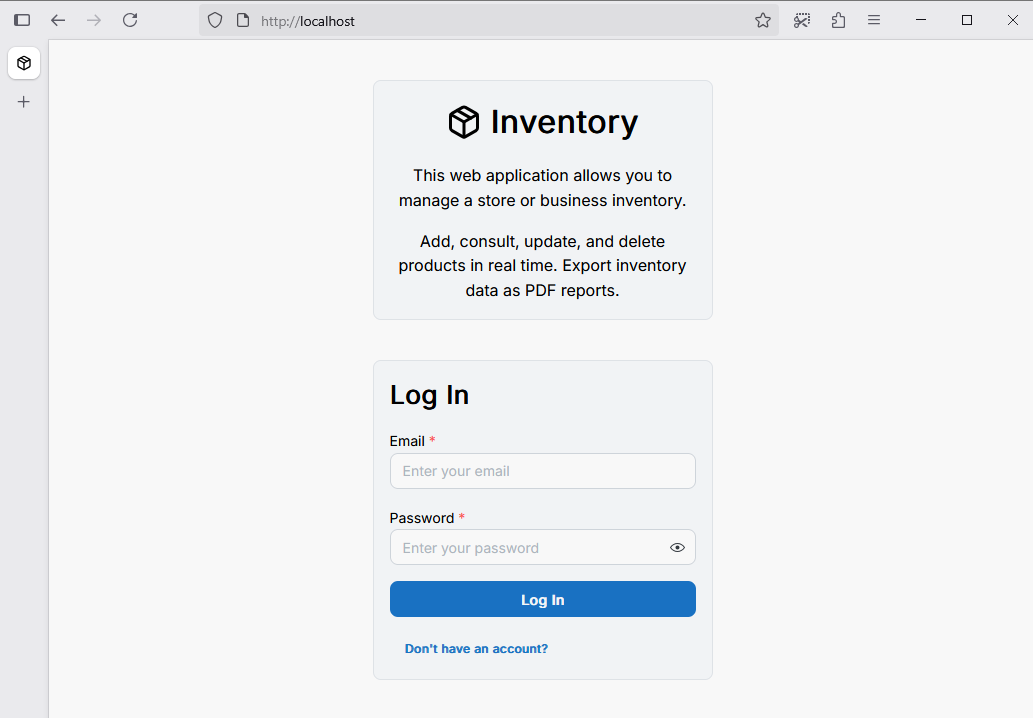
\includegraphics[width=0.95\textwidth]{images/1 Pantalla Inicial}
    \caption{Pantalla inicial de la aplicación}
\end{figure}

\subsection{Autenticación}

\subsubsection{Registro}

Inicialmente, no existe ningún usuario registrado, así que se debe registrar uno nuevo. Para ello, se da clic en el botón “Don't have an account?” y luego se debe completar el formulario de registro con un nombre de usuario, un correo electrónico y una contraseña. El usuario quedará registrado una vez que se haga clic en el botón “Register”, redirigiendo a la pantalla de inventario que se verá más adelante.

\begin{figure}[H]
    \centering
    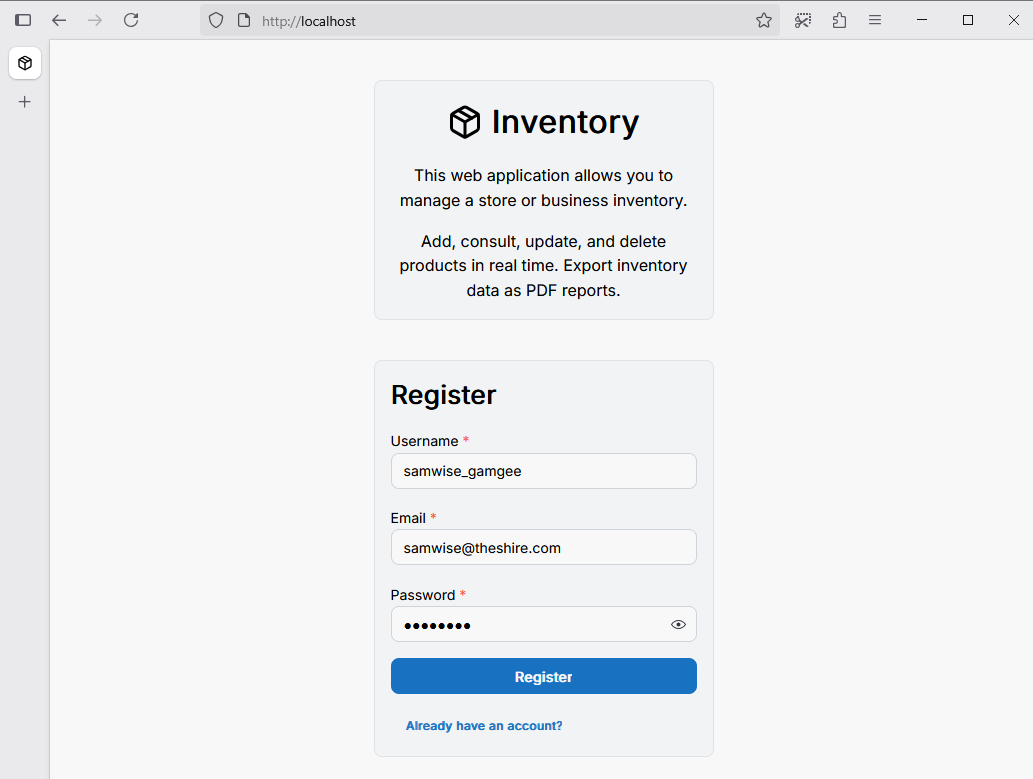
\includegraphics[width=0.95\textwidth]{images/2 Registro}
    \caption{Formulario de registro de usuario}
\end{figure}

\subsubsection{Inicio de Sesión}

Cuando un usuario ya está registrado, puede iniciar sesión simplemente ingresando su correo electrónico y contraseña en el formulario correspondiente, que aparece por defecto al ingresar la aplicación. Al hacer clic en el botón “Login”, se redirigirá a la pantalla de inventario. Para acceder a este formulario desde el formulario de registro, basta con darle clic al botón “Already have an account?”.

\begin{figure}[H]
    \centering
    \includegraphics[width=0.95\textwidth]{images/3 Inicio de Sesión}
    \caption{Formulario de inicio de sesión}
\end{figure}

\subsection{Inventario}

Después de registrarse o iniciar sesión, se redirige al usuario a la pantalla de inventario.

\begin{figure}[H]
    \centering
    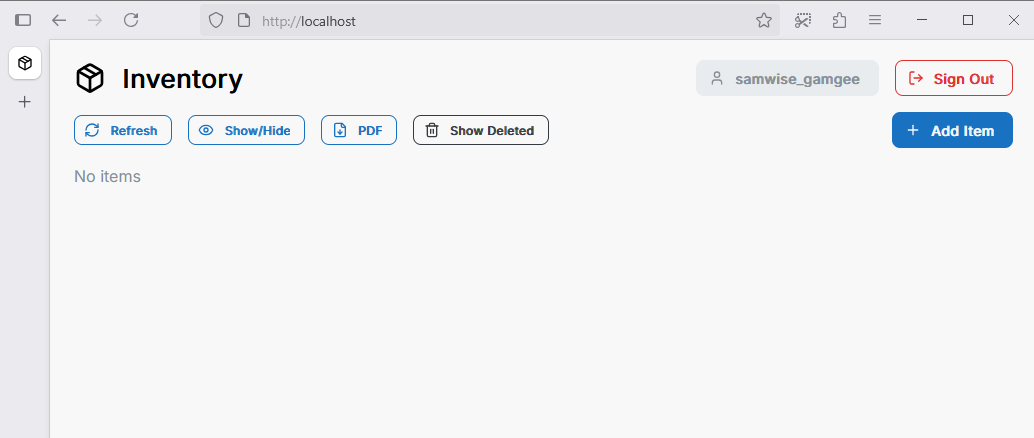
\includegraphics[width=0.95\textwidth]{images/4 Inventario}
    \caption{Pantalla principal de inventario}
\end{figure}

En esta pantalla es donde se lleva a cabo la gran parte de la funcionalidad del sistema. En la parte superior, se encuentra el nombre de la aplicación, el nombre del usuario actualmente autenticado y un botón para cerrar sesión. En la parte inferior, se muestra una tabla con los ítems que se encuentran en el inventario, que inicialmente está vacía.

Arriba de la tabla, aparecen algunos controles para manipularla o interactuar con el sistema. Estos controles son, de izquierda a derecha:

\begin{itemize}
    \item Un botón para actualizar la vista de la tabla.
    \item Un botón para elegir qué campos se desean mostrar en la tabla.
    \item Un botón para exportar la vista actual de la tabla a un archivo PDF.
    \item Un botón para mostrar los ítems eliminados.
    \item Un botón para agregar un nuevo ítem al inventario.
\end{itemize}

\subsubsection{Cierre de Sesión}

Para cerrar sesión, basta con darle clic al botón “Sign Out”, lo que redirigirá a la pantalla inicial donde los usuarios se pueden auntenticar.

\begin{figure}[H]
    \centering
    \includegraphics[width=0.95\textwidth]{images/5 Cierre de Sesión}
    \caption{Cierre de sesión}
\end{figure}

\subsubsection{Agregar ítem}

Para agregar un nuevo ítem al inventario, se debe hacer clic en el botón “Add Item”. Esto abrirá un formulario donde se deben completar los campos requeridos: nombre,SKU, descripción, precio y cantidad. Una vez completados, se debe hacer clic en el botón “Add” para guardar el nuevo ítem en la base de datos.

\begin{figure}[H]
    \centering
    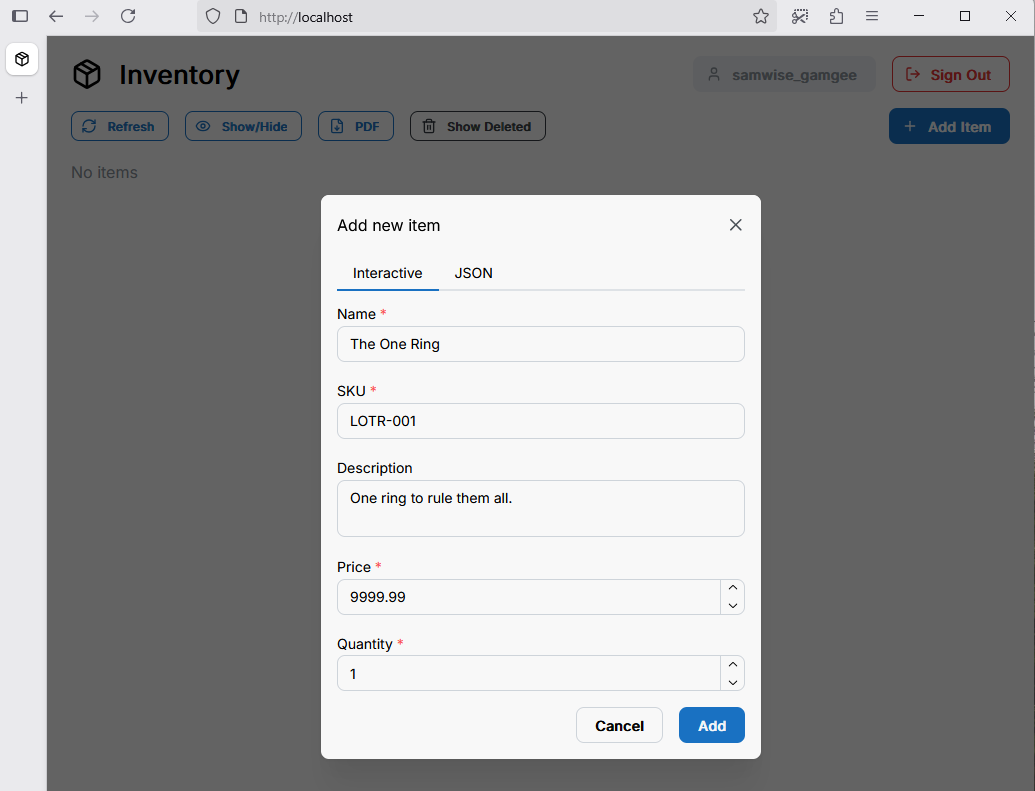
\includegraphics[width=0.95\textwidth]{images/6 Agregar}
    \caption{Formulario para agregar ítem}
\end{figure}

También existe la opción de insertar directamente estos campos en un formato JSON, seleccionando la pestaña correspondiente.

\begin{figure}[H]
    \centering
    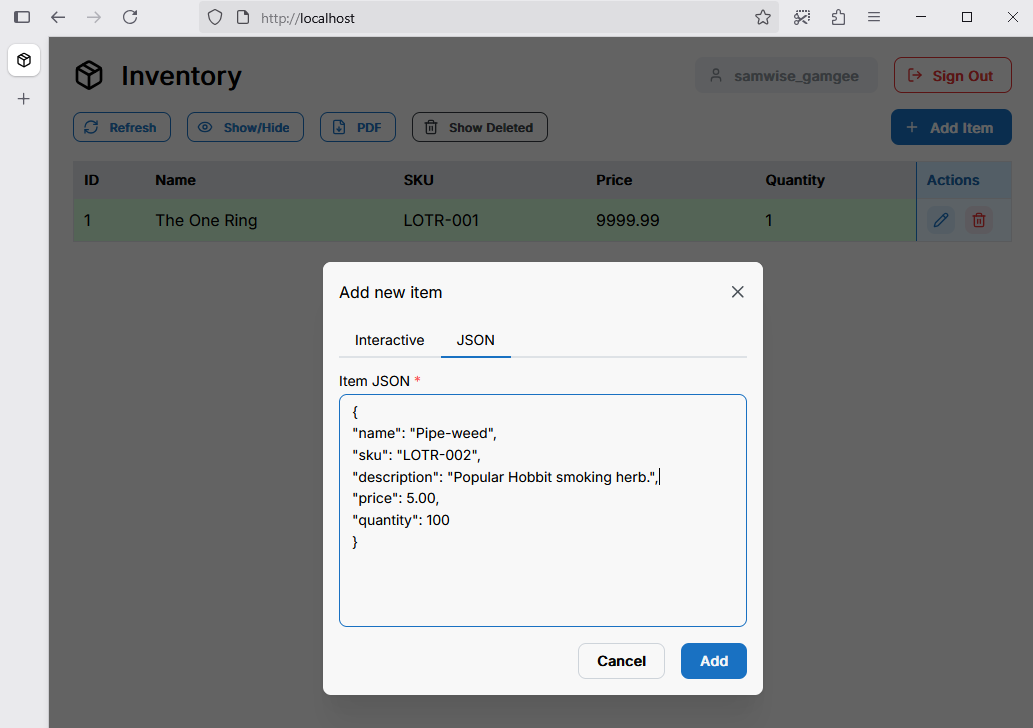
\includegraphics[width=0.95\textwidth]{images/7 Agregar JSON}
    \caption{Agregar ítem usando JSON}
\end{figure}

Los ítems agregados aparecen en color verde.

\begin{figure}[H]
    \centering
    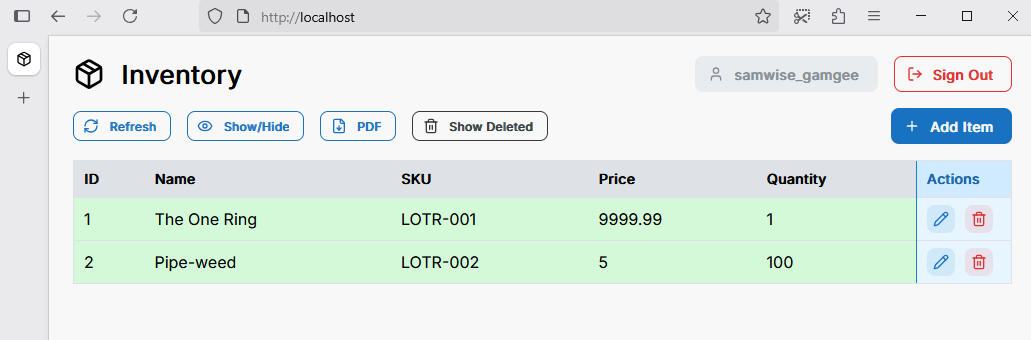
\includegraphics[width=0.95\textwidth]{images/8 Agregado}
    \caption{Ítem agregado exitosamente}
\end{figure}

Si existe algún impedimento para agregar el ítem, se le notificará al usuario. Por ejemplo, si el SKU ya existe o si el JSON no es válido.

\begin{figure}[H]
    \centering
    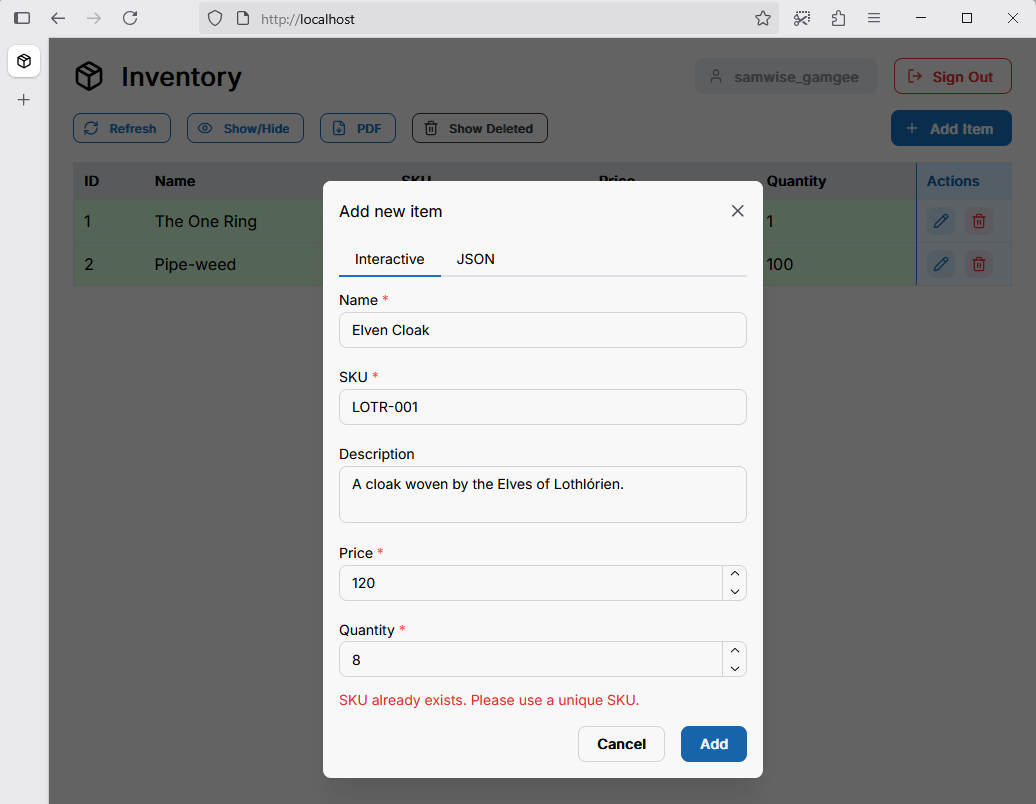
\includegraphics[width=0.95\textwidth]{images/9 Agregar Error}
    \caption{Error al agregar ítem}
\end{figure}
\begin{figure}[H]
    \centering
    \includegraphics[width=0.95\textwidth]{images/10 Agregar Error JSOn}
    \caption{Error al agregar ítem con JSON inválido}
\end{figure}

Una vez que ya se tiene al menos un ítem en el inventario, al final de cada fila aparecen dos botones: uno para editar y otro para eliminar.

\begin{figure}[H]
    \centering
    \includegraphics[width=0.95\textwidth]{images/11 Varios Ítems}
    \caption{Inventario con varios ítems}
\end{figure}

\subsubsection{Elegir Columnas Mostradas}

Es posible darle clic al botón “Show/Hide” para cambiar las columnas mostradas.

\begin{figure}[H]
    \centering
    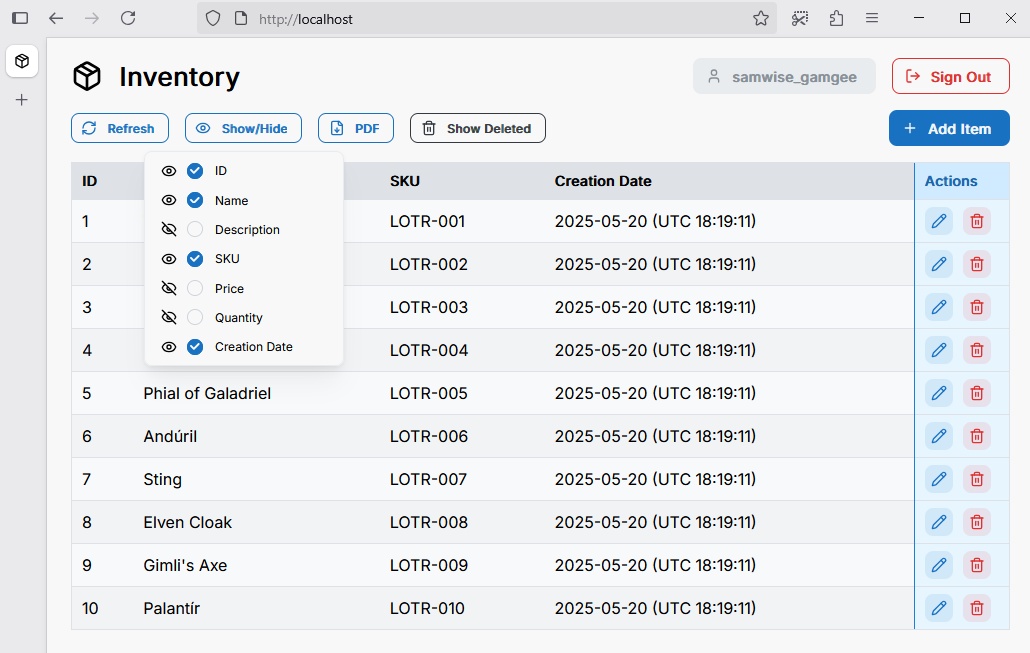
\includegraphics[width=0.95\textwidth]{images/12 Campos Mostrados}
    \caption{Selección de columnas mostradas}
\end{figure}

\subsubsection{Editar ítem}

Para editar un ítem existente, se debe hacer clic en el botón de editar correspondiente a la fila del ítem que se desea modificar. Después de hacerlo, la fila cambiará, permitiendo editar los campos que se permiten modificar (todos a excepción de ID, SKU y Creation Date).

\begin{figure}[H]
    \centering
    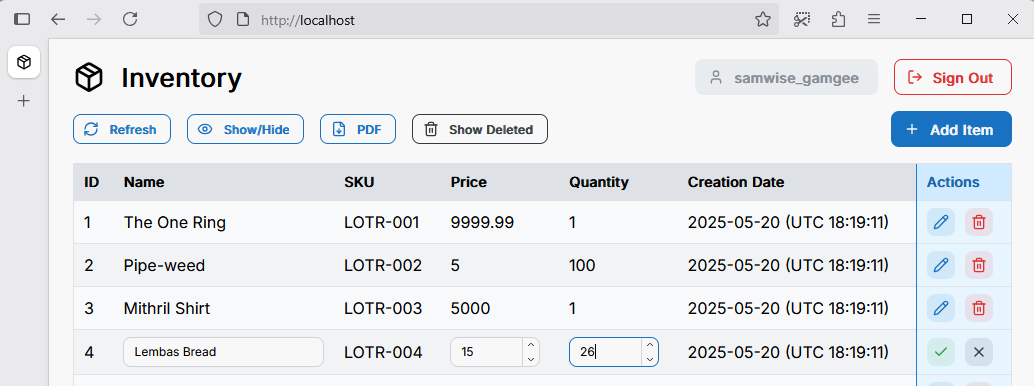
\includegraphics[width=0.95\textwidth]{images/13 Editar}
    \caption{Vista de edición}
\end{figure}

Una vez que se han hecho los cambios deseados, se pueden cancelar o enviar haciendo clic en los botones correspondientes, al final de la fila. Si enviamos los cambios, se solicita una confirmación.

\begin{figure}[H]
    \centering
    \includegraphics[width=0.95\textwidth]{images/14 Editar Confirmación}
    \caption{Confirmación de edición}
\end{figure}

Después de confirmar, podemos verificar que la información cambió y que la fila cambió a color azul.

\begin{figure}[H]
    \centering
    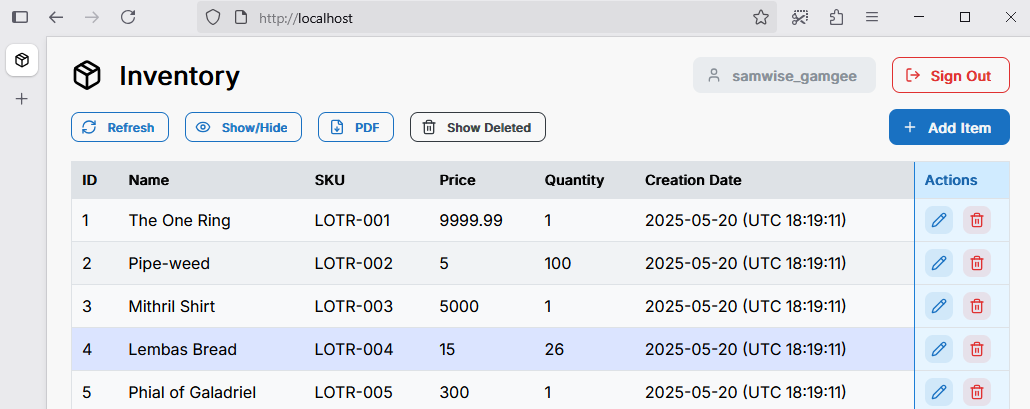
\includegraphics[width=0.95\textwidth]{images/15 Fila Editada}
    \caption{Ítem editado (color azul)}
\end{figure}

\subsubsection{Eliminar ítem}

Para eliminar un ítem, se debe hacer clic en el botón de eliminar en la fila correspondiente. Después de hacerlo, se solicitará una confirmación para proceder con la eliminación.

\begin{figure}[H]
    \centering
    \includegraphics[width=0.95\textwidth]{images/16 Eliminar Confirmación}
    \caption{Confirmación de eliminación}
\end{figure}

Una vez eliminado, la fila no desaparece, sino que se pone en color rojo con su texto tachadoo.

\begin{figure}[H]
    \centering
    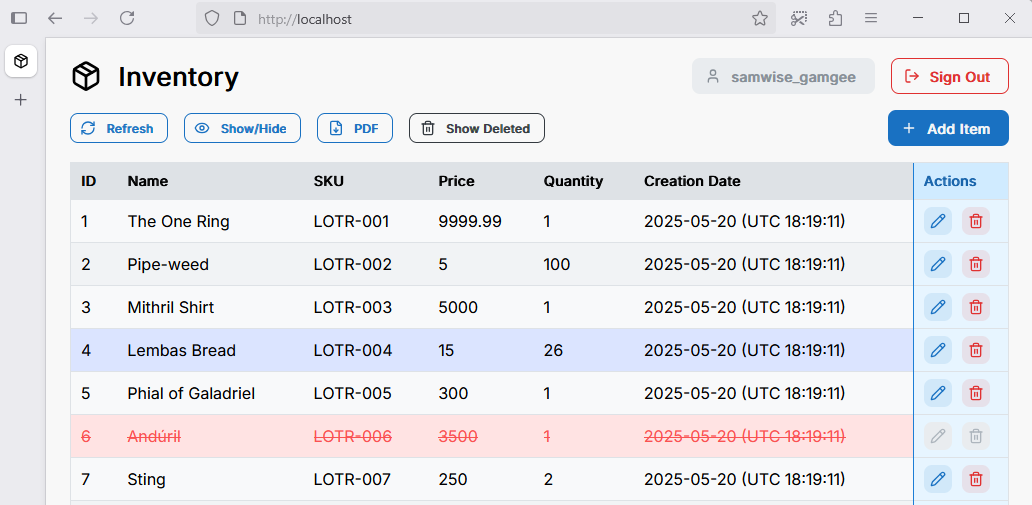
\includegraphics[width=0.95\textwidth]{images/17 Fila Eliminada}
    \caption{Ítem eliminado (color rojo)}
\end{figure}

\subsubsection{Actualizar la Vista}

Hasta ahora, hemos visto que las filas de los objetos agregados, modificados y eliminados cambian de color.

\begin{figure}[H]
    \centering
    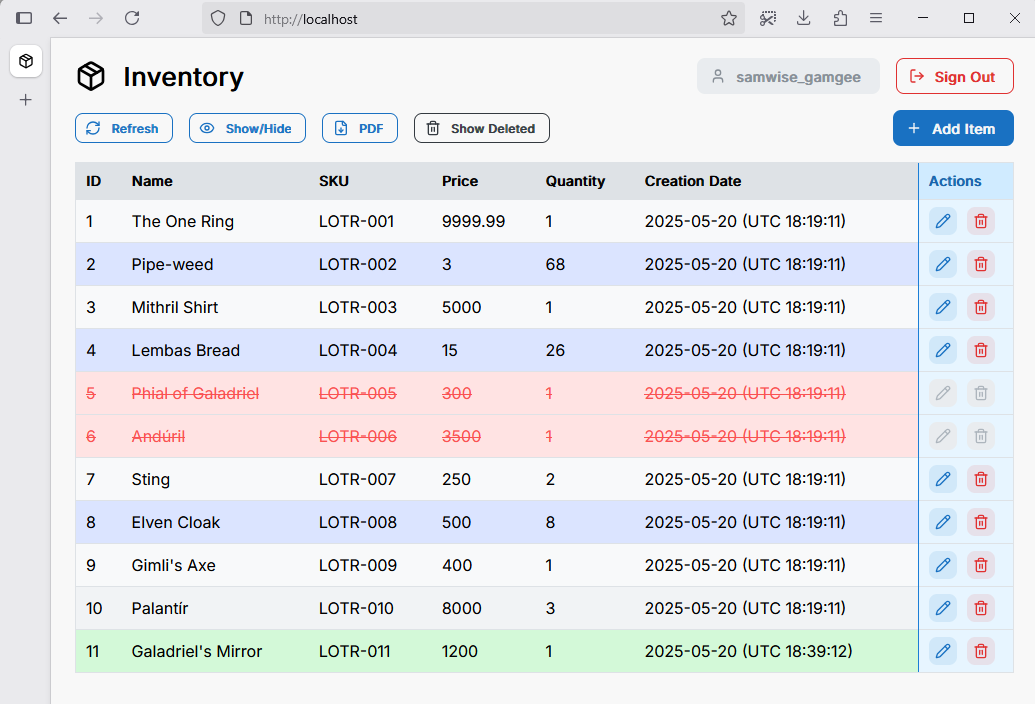
\includegraphics[width=0.95\textwidth]{images/18 Colores}
    \caption{Colores de filas según estado}
\end{figure}

Estos colores y la vista de los ítems ya eliminados son temporales. Para hacerlos desaparecer, se debe hacer clic en el botón “Refresh”.

\begin{figure}[H]
    \centering
    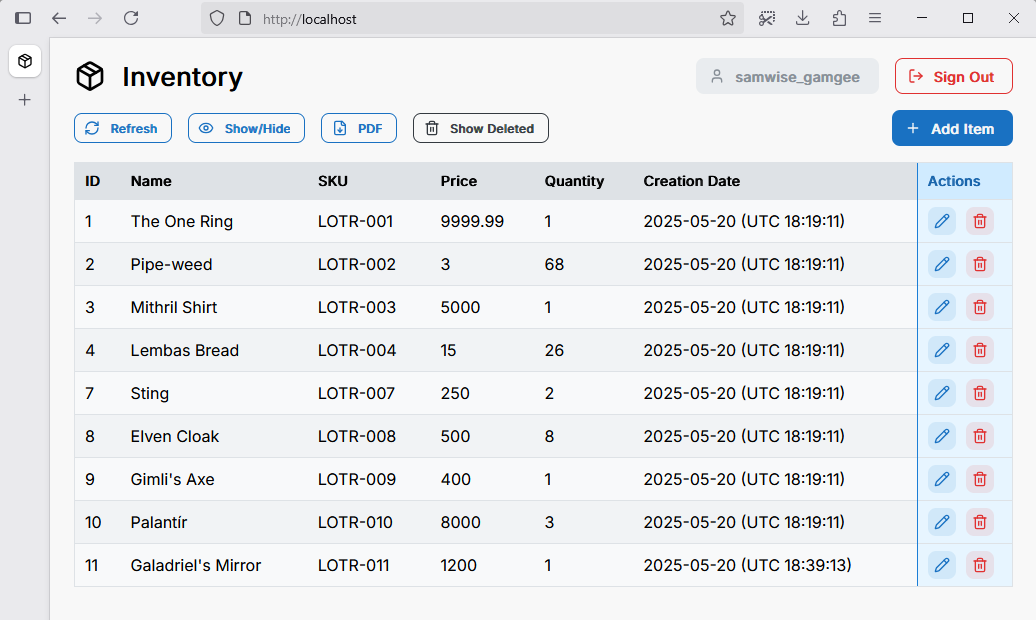
\includegraphics[width=0.95\textwidth]{images/19 Actualizado}
    \caption{Vista actualizada del inventario}
\end{figure}

Este botón también actualizará la vista, mostrando los cambios en el inventario que algún otro usuario haya hecho.

\subsubsection{Exportar a PDF}

Para exportar la vista actual de la tabla a un archivo PDF, se debe hacer clic en el botón “PDF”. Esto generará un archivo PDF con el contenido de la tabla, que se descargará automáticamente. Esta funcionalidad es especialmente útil cuando todavía tenemos los ítems manipulados en colores, pues el PDF se exporta con esos colores, permitiendo esencialmente guardar un registro de los cambios realizados.

\begin{figure}[H]
    \centering
    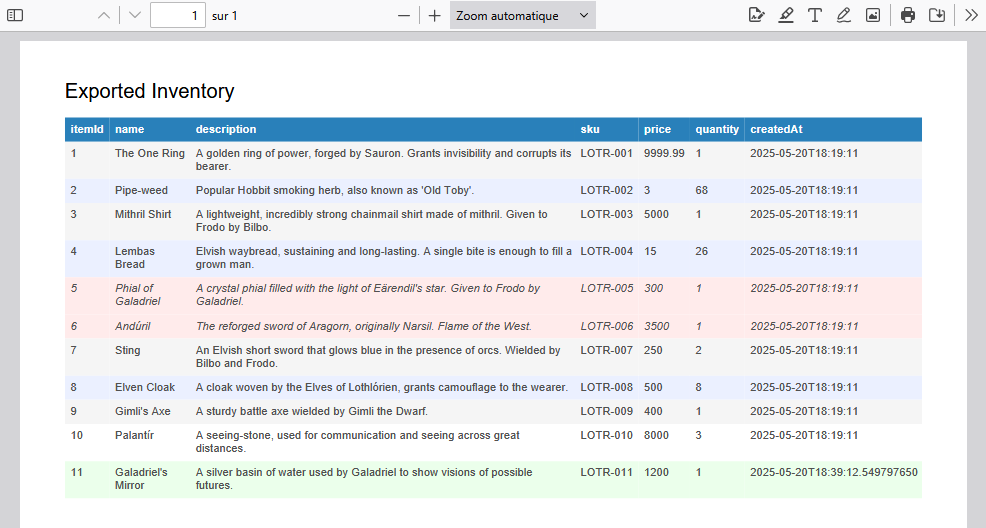
\includegraphics[width=0.95\textwidth]{images/20 PDF Colores}
    \caption{Exportación a PDF con colores}
\end{figure}

Si las filas no están coloreadas, permanecerán de esa forma.

\begin{figure}[H]
    \centering
    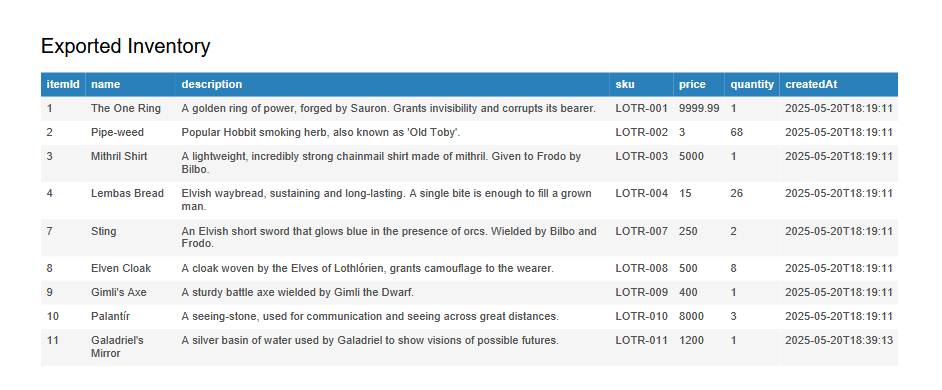
\includegraphics[width=0.95\textwidth]{images/21 PDF Actualizado}
    \caption{Exportación a PDF sin colores}
\end{figure}

\subsubsection{Restaurar ítem}

Si queremos ver los ítems que han sido eliminados, basta con darle clic al botón “Show Deleted”.

\begin{figure}[H]
    \centering
    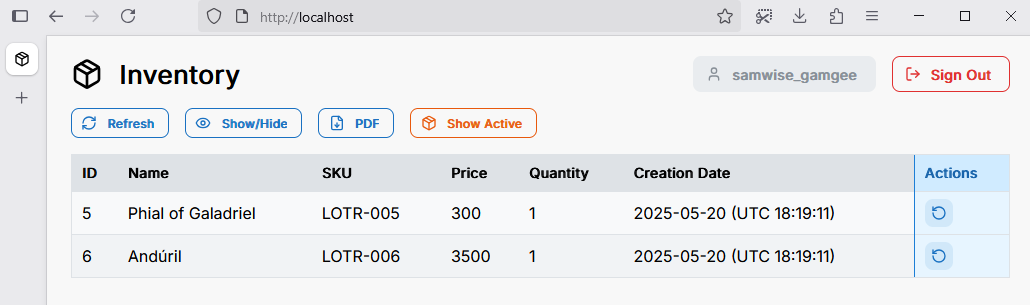
\includegraphics[width=0.95\textwidth]{images/22 Eliminados}
    \caption{Vista de ítems eliminados}
\end{figure}

Para regresar a la vista normal de los ítems activos, se da clic al botón “Show Active”.

En esta vista de ítems eliminados, se tiene la opción de restaurarlos (es decir, hacerlos activos de nuevo). Para hacerlo, se da clic al botón de restaurar que aparece al final de cada fila, pidiendo una confirmación.

\begin{figure}[H]
    \centering
    \includegraphics[width=0.95\textwidth]{images/23 Restaurar Confirmación}
    \caption{Confirmación de restauración}
\end{figure}

Los ítems restaurados aparecen en color naranja y, similar a los eliminados en la vista normal, desaparecerán una vez que se actualice la vista.

\begin{figure}[H]
    \centering
    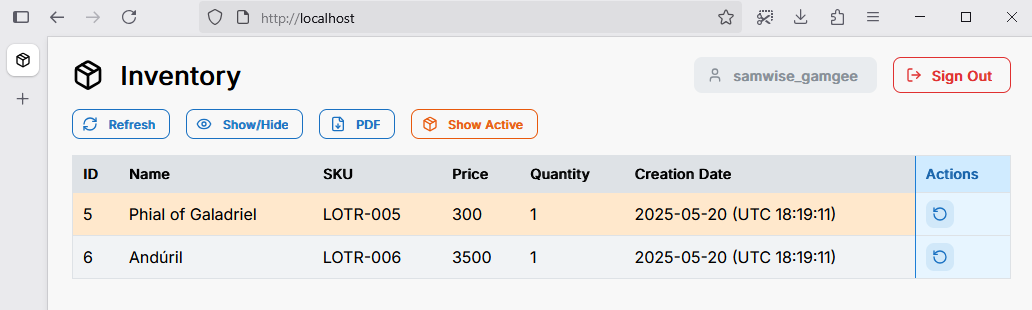
\includegraphics[width=0.95\textwidth]{images/24 Restaurado}
    \caption{Ítem restaurado (color naranja)}
\end{figure}
\begin{figure}[H]
    \centering
    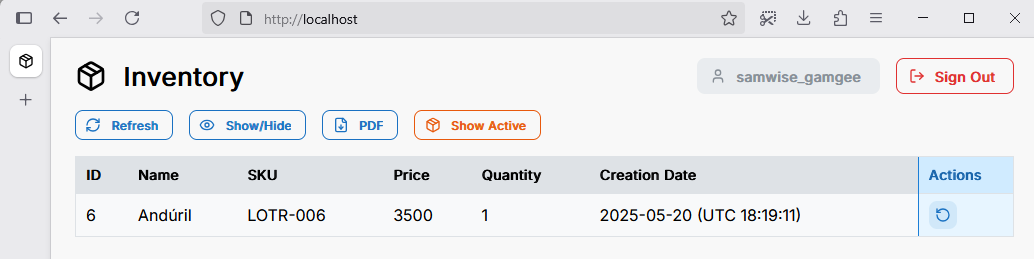
\includegraphics[width=0.95\textwidth]{images/25 Eliminados Actualizado}
    \caption{Vista de eliminados tras restaurar}
\end{figure}
